% !TeX root = ..\main.tex
%%%%%%%%%%%%%%%%%%%%%%%%%  
\section{Cấu trúc mã nguồn}
\subsection{Cấu trúc front-end}
\begin{figure}[!htp]
    \begin{center}
        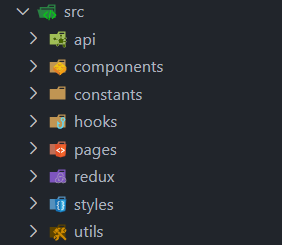
\includegraphics[width=7cm]{img/file-structure/front-end.png}
    \end{center}
    \caption{Cấu trúc mã nguồn front-end}
\end{figure}

Hệ thống thư mục bao gồm:
\begin{itemize}
    \item api: Chứa các lời gọi api đến Back-end
    \item component: Chứa các đối tượng sử dụng trong giao diện
    \item constants: Chứa các asset, các dữ liệu giá trị không thay đổi
    \item hooks: Chứa các hook sử dụng trong hệ thống
    \item pages: Chứa các giao diện trong hệ thống
    \item redux: Chứa các đối tượng sử dụng trong redux
    \item style: Chứa các file css sử dụng trong hệ thống
    \item util: Chứa các hàm hỗ trợ hệ thống, các kiểu dữ liệu, các modal,..
\end{itemize}


\subsection{Cấu trúc back-end}
\begin{figure}[!htp]
    \begin{center}
        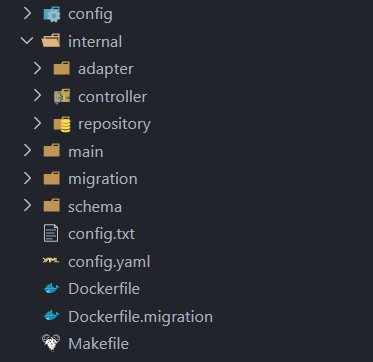
\includegraphics[width=7cm]{img/file-structure/back-end.png}
    \end{center}
    \caption{Cấu trúc mã nguồn back-end}
\end{figure}

Hệ thống thư mục bao gồm:
\begin{itemize}
    \item config: Chứa các file cấu hình dịch vụ web
    \item internal: Bao gồm các thư mục
          \begin{itemize}
              \item adapter: Chứa các file kết nối qua các dịch vụ web khác, các hệ thống khác
              \item controller: Chứa các file xử lý các tác vụ từ các yêu cầu
              \item repository: Chứa các file có nhiệm vụ tương tác trực tiếp với cơ sở dữ liệu
          \end{itemize}
    \item main: Chứa các file để khởi động các dịch vụ web
    \item migration: Chứa các file dùng để quản lý dữ liệu trên cơ sở dữ liệu
    \item schema: Chứa các struct dữ liệu được sử dụng để lưu trữ dữ liệu trong quá trình thực hiện các yêu cầu
\end{itemize}

\subsection{Cấu trúc BPEL}

\begin{figure}[!htp]
    \begin{center}
        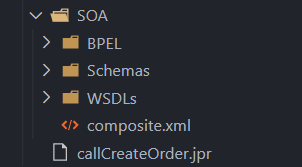
\includegraphics[width=6cm]{img/file-structure/bpel.png}
    \end{center}
    \caption{Cấu trúc mã nguồn bpel}
\end{figure}

\begin{itemize}
    \item BPEL: Chứa các file thực thi quy trình nghiệp vụ
    \item Schemas: Chứa các struct được sử dụng để lưu trữ dữ liệu trong quá trình truyền nhận dữ liệu
    \item WSDLs: Chứa các file mô tả các dịch vụ web
    \item file .jpr: File dùng để cấu hình dịch vụ web
\end{itemize}